\documentclass[11pt,a4paper]{article}

% --- packages ---
\usepackage[a4paper, top=2cm, bottom=2cm, left=2cm, right=2cm]{geometry}
\usepackage[utf8]{inputenc}        % allow é, ï, etc.
\usepackage[T1]{fontenc}           % proper text encoding
\usepackage{tikz}                  % drawing the forest plot
\usepackage{xcolor}                % named colors
\usepackage{caption}               % \captionof{figure}{...}
\usepackage{booktabs}              % \toprule, \midrule, \bottomrule
\usepackage{graphicx}              % \includegraphics
\usepackage{eurosym}               % \euro{} for euro signs
\usetikzlibrary{arrows.meta, positioning, fit}

% tighten paragraph spacing for the page budget
\setlength{\parskip}{4pt plus 1pt minus 1pt}
\setlength{\parindent}{0pt}

% figures generated by the notebook live here
\graphicspath{{reporting/figures/}}

% --- custom colors used in the figure ---
\definecolor{accent}{HTML}{2E5C8A}    % blue
\definecolor{accent2}{HTML}{4C9A4A}   % green (v3 — causally identified)
\definecolor{accent3}{HTML}{C04848}   % red (v1 — wrong sign)
\definecolor{accent4}{HTML}{E0B341}   % amber (v4, v5 — over-controlled)

\title{Dynamic Pricing for European Camping Group}
\author{Jimmy Zhang, Tobias Vanoverschelde, Fausto De Valck, Andrew Posey,
Alexander Lievens \\ KU Leuven, Statistical Consulting 2025-2026, ORTEC Project}
\date{May 2026}

\begin{document}
\maketitle

\section{Problem and Business Context}

European Camping Group (ECG) operates over 400 campsites across 10 European countries with several accommodation types and four distinct market segments. With a 30 week open season, this is more than 250{,}000 individual prices to set every year, one for every combination of campsite, accommodation, market, and arrival week. We refer to such a combination as a \emph{ROMGID} (reservable option market group), the unit of analysis throughout the report. Based on the information and business case provided, this report will examine the following question. Can historical booking data be used to recommended better prices for ROMGID’s and increase ECG’s revenue?

\section{The Trap}

The most direct approach, regressing booked nights on price while controlling for accommodation and seasonality, yields an answer that is economically impossible. On a 50{,}000 row training sample, the estimated price coefficient is positive: $\beta = +0.29$, with an 80\% credible interval of $[+0.18, +0.42]$. Read literally, this means ``raising prices increases bookings''.

The reason is structural, not statistical. ECG's pricing system already reacts to demand: when a campsite fills up, prices rise, when bookings slow down, prices fall. Due to this, high prices and high bookings tend to occur together in the data, not because price causes bookings, but because both respond to a common, unobservable underlying demand signal.

The fix requires identifying this demand signal that the pricer reacts to. Bookings on books (BoB), the total number of nights a ROMGID has previously been reserved when a price is set. Including this variable in the model helps remove historical booking bias and better isolate the true impact of price on individuals’ bookings.

\begin{center}
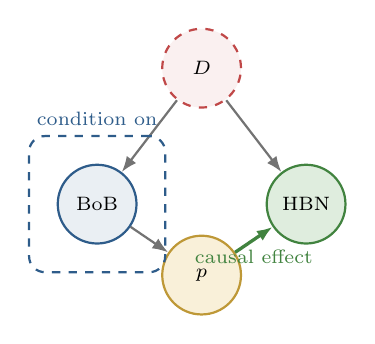
\begin{tikzpicture}[
  obs/.style={circle, draw=accent, thick, fill=accent!10, minimum size=10mm, font=\scriptsize, inner sep=0pt},
  latent/.style={circle, draw=accent3, thick, dashed, fill=accent3!8, minimum size=10mm, font=\scriptsize, inner sep=0pt},
  treatment/.style={circle, draw=accent4!85!black, thick, fill=accent4!20, minimum size=10mm, font=\scriptsize, inner sep=0pt},
  outcome/.style={circle, draw=accent2!85!black, thick, fill=accent2!18, minimum size=10mm, font=\scriptsize, inner sep=0pt},
  arrow/.style={-{Latex[length=2mm]}, thick, draw=black!55},
  causal/.style={-{Latex[length=2mm]}, thick, draw=accent2!85!black, line width=1.2pt},
]
\node[latent]    (D)                                       {$D$};
\node[obs]       (BoB) [below left=10mm and 6mm of D]      {BoB};
\node[treatment] (P)   [below=16mm of D]                   {$p$};
\node[outcome]   (Y)   [below right=10mm and 6mm of D]     {HBN};

\draw[arrow]  (D)   -- (BoB);
\draw[arrow]  (BoB) -- (P);
\draw[arrow]  (D)   -- (Y);
\draw[causal] (P)   -- (Y) node[midway, below, font=\scriptsize, color=accent2!85!black] {causal effect};

% Highlight that we condition on BoB
\node[draw=accent, thick, dashed, rounded corners=2mm, inner sep=3.5mm,
      fit=(BoB), label={[font=\scriptsize, color=accent]above:condition on}] {};
\end{tikzpicture}
\captionof{figure}{Causal structure linking price ($p$) and bookings (HBN). Latent demand $D$ (red, dashed, unobservable) drives bookings on books (BoB, observed) and bookings directly. The existing pricer sets $p$ in response to BoB. The path $p \leftarrow \mathrm{BoB} \leftarrow D \to \mathrm{HBN}$ is a problem: it lets demand contaminate the apparent price to bookings relationship. Conditioning on BoB (dashed blue box) removes this, leaving only the genuine causal effect $p \to \mathrm{HBN}$.}
\end{center}

\smallskip

\begin{center}
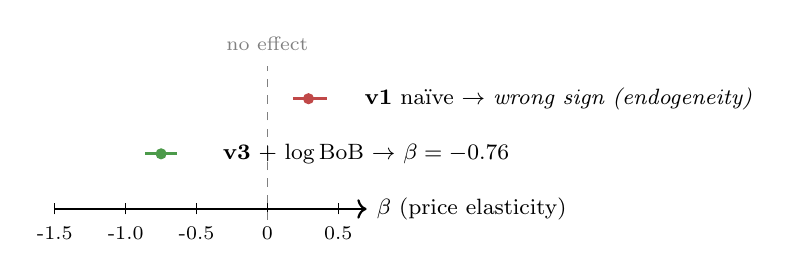
\begin{tikzpicture}[x=18mm, y=7mm]
  % axis (zoomed in to v1 / v3 range)
  \draw[->, thick] (-1.5, 0) -- (0.7, 0) node[right, font=\footnotesize] {$\beta$ (price elasticity)};
  \foreach \x in {-1.5, -1.0, -0.5, 0, 0.5} {
      \draw (\x, -0.1) -- (\x, 0.1);
      \node[below, font=\scriptsize] at (\x, -0.15) {\x};
  }
  \draw[dashed, gray] (0, -0.2) -- (0, 2.6);
  \node[gray, font=\scriptsize, above] at (0, 2.7) {no effect};

  % v1 — naïve, wrong sign
  \draw[thick, accent3, line width=1pt] (0.18, 2.0) -- (0.42, 2.0);
  \filldraw[accent3] (0.29, 2.0) circle (1.8pt);
  \node[right=3mm, font=\footnotesize] at (0.45, 2.0) {\textbf{v1} naïve $\to$ \emph{wrong sign (endogeneity)}};

  % v3 — conditioned on log_bob
  \draw[thick, accent2, line width=1pt] (-0.86, 1.0) -- (-0.64, 1.0);
  \filldraw[accent2] (-0.75, 1.0) circle (1.8pt);
  \node[right=3mm, font=\footnotesize] at (-0.55, 1.0) {\textbf{v3} $+\,\log\mathrm{BoB}$ $\to$ \emph{$\beta = -0.76$}};
\end{tikzpicture}
\captionof{figure}{Posterior point estimate and 80\% credible interval for the global price elasticity $\beta$. The naïve specification (v1) proposes an economically impossible impact, direct evidence of the correlation between price and bookings in ECG's data. After conditioning on BoB, the elasticity becomes negative as economic theory requires (v3, $\beta = -0.76$).}
\end{center}

\section{Two Models, Two Jobs}

The Bayesian estimate of $\beta = -0.76$ from model v1 implies demand is inelastic on average ($|\beta| < 1$). This means that for every 1\% increase in price, bookings decrease by around 0.76\%. Because this response is less than proportional, total revenue (price multiplied by bookings), on average, goes up when prices go up, within the price range our data cover. Under a constant elasticity assumption, this would mean ECG could raise prices and capture more revenue. Based on this learning, we created an improved gradient boosted trees model (LightGBM) optimiser, referenced in Section 4, that helps clarify our understanding. Average elasticity across ROMGIDs is correct, but the per ROMGID optimal price is varied. Some sites are overpriced, some are underpriced, and the total sum of movements is close to zero. Therefore, the pricing engine should focus on specific sites, rather than all sites collectively, to adjust prices on in order to maximize revenue.

Model v3 is intentionally minimal as it only uses the variables strictly needed to remove the impact of BoB. Through this minimalism, it is an effective estimator of the local average elasticity, but it is unable to make future predictions. To predict bookings at a specific time and price, we trained a LightGBM model on the same conditions as before but included lead time and calendar and accommodation features that were intentionally left out of v3. Trees were chosen for this model because they will not overfit when multiple variables are included unlike some Bayesian models. At typical prices, this LightGBM model produced the same beta as the Bayesian model (around $-0.75$). This brings validity to our elasticity value as two different models with different assumptions resulted in the same answer.

Out of sample, LightGBM achieves a median ROMGID level error of 27\% on total booked nights, which is within reason for the industry. This error is concentrated in low volume ROMGID's where small absolute differences in bookings inflate percentage errors. For ROMGID's with at least 10 bookings per season, the median error drops to 22\%.

\section{The Optimiser and What It Recommends}

For each tested snapshot independently, we ask the LightGBM forecaster a question, at this point in the booking horizon, what price would have produced the highest predicted revenue? We simulated 21 different price points, ranging between up to 15\% higher or lower than historical rates, to determine the exact price that maximises predicted revenue. Therefore, for every ROMGID, the output is 53 prices across the total booking horizon, one per snapshot.

Three constraints keep the recommendation logical. The potential range is capped at $\pm 15\%$ of historical prices for each ROMGID, predicted bookings are can only reach capacity and nothing further, and every recommendation passes through a two tier flag (green / yellow) system before deployment, keeping humans in the loop.

\newpage Applied to 14{,}200 ROMGID's in the held out test fold:

\begin{center}
\small
\begin{tabular}{@{}lr@{}}
\toprule
\textbf{Metric} & \textbf{Value} \\
\midrule
Median per ROMGID $\Delta$price & $-0.7\%$ \\
$\Delta$price IQR (per ROMGID) & $[-6.0\%,\, +5.4\%]$ \\
\% snapshots at upper bound (1.15$\times$) & 12.7\% \\
\% snapshots at lower bound (0.85$\times$) & 14.7\% \\
\% snapshots with interior optimum & \textbf{72.6\%} \\
Total predicted uplift & \euro{}63M \\
Uplift as \% of baseline & $+38.8\%$ \\
Flag split (green / yellow) & 51\% / 49\% \\
\bottomrule
\end{tabular}
\end{center}

\begin{center}
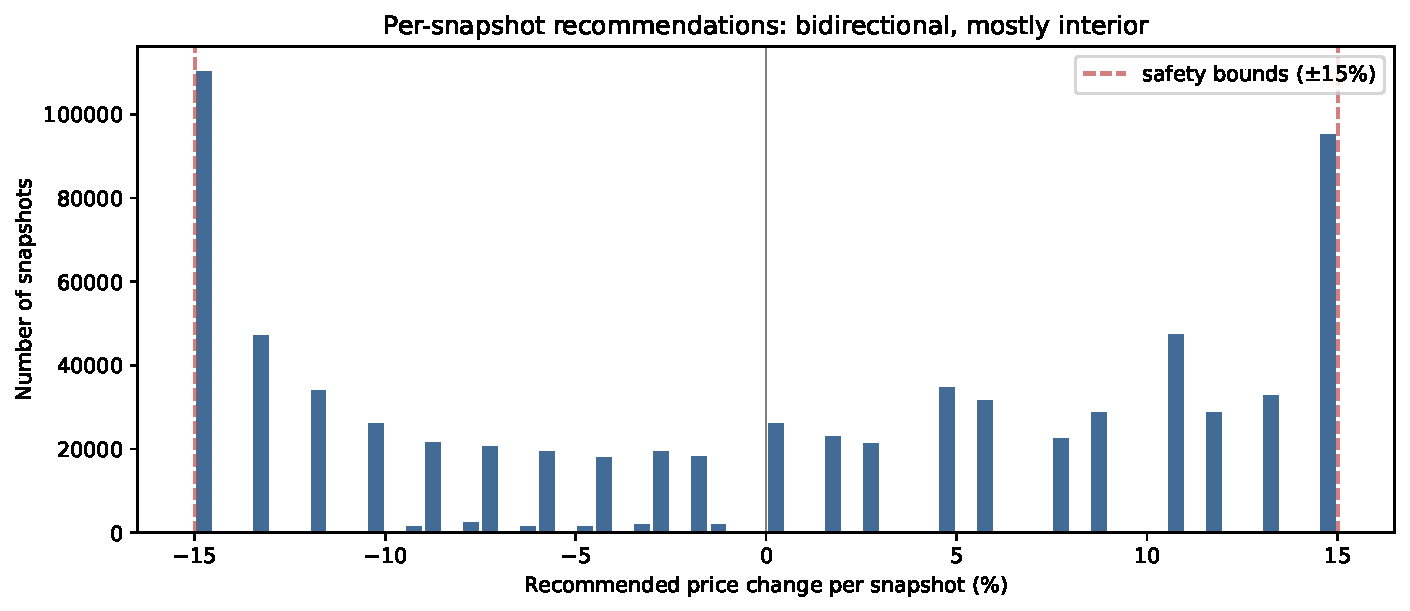
\includegraphics[width=0.7\linewidth]{recommendations_distribution.pdf}
\captionof{figure}{Distribution of recommended price changes across all test fold snapshots. The histogram is roughly symmetric around zero, with mass at both the lower and upper safety bounds. About 73\% of decisions land at an interior optimum within the safety bounds, 14.7\% land at a 15\% discount, and 12.7\% land at a 15\% increase.}
\end{center}

The most important number on the above figure is the \textbf{72.6\% interior optimum rate}. For nearly three quarters of snapshot decisions, the model finds a revenue maximising price strictly inside the $\pm 15\%$ safety bounds, not at a boundary. This is something that the constant elasticity Bayesian model in Section 2 could not produce. When elasticity is forced to be constant, the revenue function has no interior maximum since an increase in price will always increase revenue, but when LightGBM develops a flexible price demand curve, genuine interior optima emerge. The recommendations are also bidirectional as both price increases and decreases are promoted. From this model, ECG is overpricing some cells and underpricing others, with the majority of decisions sitting at modest price adjustments.

\begin{center}
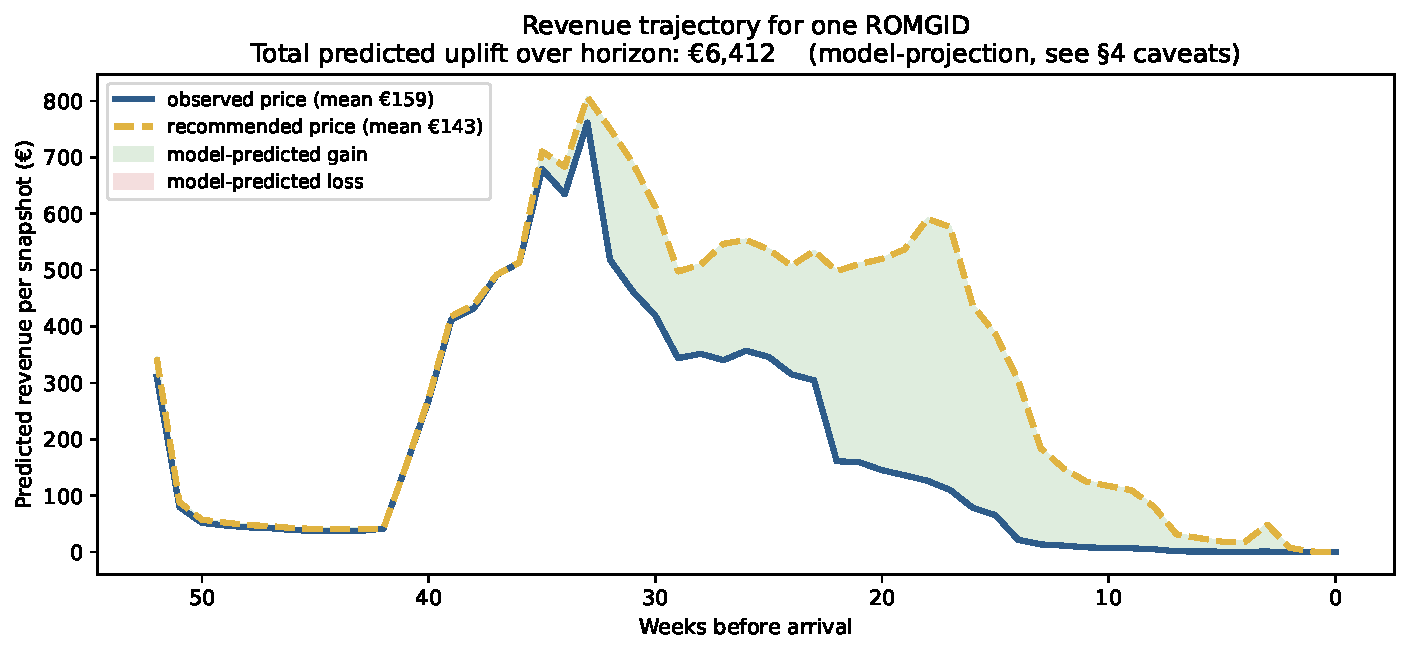
\includegraphics[width=0.7\linewidth]{revenue_trajectory.pdf}
\captionof{figure}{Predicted revenue per snapshot for one representative ROMGID, observed price (blue) versus recommended price (amber), with 80\% prediction intervals from a quantile LightGBM. Most of the booking horizon shows similar predicted revenue under both strategies, with the recommended trajectory slightly higher in the mid horizon weeks where the majority bookings actually concentrate.}
\end{center}

The +\euro{}63M total predicted uplift is a model projection and is likely optimistic for three reasons. First, the model has a 27\% out of sample error on observed prices, and utilizing predicted prices pushes it further from historical data. Second, the optimiser picks the candidate that maximises predicted revenue, exploiting any potential model error that may occur. Third, the model can predict on small positive bookings in late horizon snapshots, where historical bookings are almost zero, and then sees these bookings as small revenue gains. While the directional adjustments of the model are robust, the magnitude of the price changes is not. Therefore, a randomised price experiment, discussed in the next section, is the best way to improve the validity of the model for ECG.

\section{What ECG Should Do Next}

Two complementary tracks are recommended by this report. The first will validate the magnitude of price adjustment for the model, and the second will implement the model pipeline alongside the dashboard.

\paragraph{1. Run a small randomised price experiment.} The +\euro{}63M figure is a model projection, not a verified lift estimate. The three reasons it is optimistic, listed at the end of Section 4, cannot be resolved by further analysis of the historical data. They can only be resolved by generating new data under a known, randomised intervention. We recommend selecting 100 to 200 ROMGID's across markets and accommodation types, randomising their price by $\pm 25\%$ over a single 30 week season, and observing the resulting bookings. This experiment will highlight two things. One, it will provide an unbiased elasticity estimate that can be used to refit the model. Second, it will test for conditions greater than the $\pm 15\%$ safety range that it was developed under. While this experiment could temporarily lower the income from the selected sites, it will produce data for a stronger model with an improved pricing recommendation system.

\paragraph{2. Run the pipeline alongside the experiment.} The pipeline produces a \texttt{recommendations.csv} every time it runs, with one row per ROMGID containing the current price, recommended price, predicted bookings, revenue uplift with an 80\% credible interval, and an intervention flag. Because the model conditions on BoB at the moment of prediction, any new reservation that enters ECG's booking system automatically shifts the ROMGID to a different point on the demand curve. Therefore, a nightly rerun will need to be done for all active ROMGIDs to update the features and prices.  After the update, the file will be regenerated so the dashboard remains up to date without having to retrain the model. Model retraining will only occur once per season once a full year’s worth of data is available to update the estimates of elasticity.

The prototype dashboard delivered alongside this report reads the recommendation file and presents each ROMGID as a row in a sortable, filterable table. A pricing manager would open the dashboard and see, for every campsite week combination, the current price, the model's recommended price, the percentage change, the predicted revenue uplift, and a colour coded flag. Clicking a row would create a detail panel with observed versus predicted bookings, a capacity utilisation bar, historical price volatility, and a plain language explanation of why the recommendation was flagged the way it was.

\begin{center}
\small
\begin{tabular}{@{}llllrrr@{}}
\toprule
\textbf{ROMGID} & \textbf{Campsite} & \textbf{Type} & \textbf{Flag} & \textbf{Current} & \textbf{Recommended} & \textbf{$\Delta$price} \\
\midrule
0042 & CS-FR-118 & Mobile Home & \colorbox{accent4!25}{yellow} & \euro{}187 & \euro{}164 & $-12.3\%$ \\
\bottomrule
\end{tabular}
\captionof{figure}{Example row from the pricing dashboard. This ROMGID is flagged yellow because the recommended adjustment exceeds 10\%; therefore, the pricing manager would review local context before approving.}}
\end{center}

The flag system connects the model to the human. A \textbf{green} flag means the recommended adjustment is small (at most 10\%) and the historical price has been stable (coefficient of variation below 0.15). A \textbf{yellow} flag means the adjustment is larger (10--20\%) or the historical price has been moderately volatile. A yellow flag does not indicate that the prediction is wrong, it means a manager needs to check for what the model cannot forecast. Examples of this would be a local festival is happening nearby or a weather front is incoming. Yellow flagged ROMGIDs will be queued for the manager to review daily.

\paragraph{Why Both Tracks are Necessary.} The two tracks answer different questions. The first track validates the \emph{magnitude} of the recommended adjustments by creating predicted prices that cannot be provided by the historical data. The second track builds the \emph{managerial trust} required for adoption by letting the team compare the engine's suggestions against their own decisions over a season. This will help the team develop a feel for where the model adds value, and where their expertise will remain essential. Automatic price adjustments based on green flag recommendations should only begin once the experiment confirms the elasticity at the ROMGID level, and the managers believe the recommendations from the pipeline are sensible. Until the data from the experiment are available, every recommendation will be advisory. Once the data are in and the managers understand the recommendations, the manager will move from updating all prices, to auditing unexpected price changes thereby utilizing their domain knowledge in a more targeted fashion.

\paragraph{Limitations.} The methodology rests on three assumptions worth flagging:
\begin{itemize}
    \item \textbf{Unobserved Errors:} While we close the primary correlation bias, (demand autocorrelation via $\log\mathrm{BoB}$), other sources of price errors, such as sudden campsite changes or manual manager overrides, remain unobservable in this dataset.
    \item \textbf{Model Exploitation:} LightGBM's 27\% out of sample error naturally grows for predictive prices that are not in the historical data. The optimiser may "exploit" this noise, picking prices that appear optimal due to prediction error rather than true demand response.
    \item \textbf{Capacity Constraints:} Capacity is realistically nonbinding in much of the dataset (median utilization 10\%). A real deployment in peak weeks at premium properties would likely encounter the capacity constraint that is currently a tested but inactive safeguard.
\end{itemize}

\section{Conclusion}

Treating dynamic pricing as a cause and effect problem creates a clear correlation trap. Once this problem is avoided, a local elasticity of $-0.76$ can be found. A LightGBM forecaster delivers per snapshot recommendations that are both bidirectional and different in magnitude for each ROMGID. This results in a pipeline that includes a recommendation file, a review workflow dashboard based on a flagging mechanism, and an integration plan where the experiment verifies the elasticity and the recommendations are verified by the managerial team. This process will integrate the managers in the decision process and build trust with them. This system will not replace the pricing manager, but will instead focus their attention on specific ROMGIDs that need domain expertise.

As it stands, ECG is leaving money on the table. While the true amount cannot be verified by this report, a small randomised experiment alongside a deployment of the validation pipeline will answer it with minimal cost.


\end{document}
